
\section{Implementation and Case Study}
We present \textbf{D-Hammer}, an open-source and publicly
available\footnote{{\textcolor{red}{URL}}} implementaion of our
approach.  \textbf{D-Hammer} is an equational prover for Labelled
Dirac notation written in \CC.  It features a parser built using
ANTLR4, and scalar reasoning is powered by the Mathematica
Engine. Users can use commands to make definitions and assumptions in
the maintained context, conduct the normalization and equivalence
checking, and obtain the rewriting trace output.  D-Hammer can be run
interactively from the command line or integrated into other
\CC\ projects as a library.


\subsubsection{Structure and Mechanism} 
The project consists of the following components:
\begin{itemize}
    \item \texttt{antlr4}: A third-party library for building the parser.
    \item \texttt{WSTP interface}: A wrapper to link with Mathematica Engine.
    \item \texttt{ualg}: The framework module for universal algebra, defining basic concepts like terms and substitutions.
    \item \texttt{dhammer}: The main module containing symbols definitions, type checking, rewriting rules, normalization algorithm and the prover.
    \item \texttt{example}: An example benchmark for evaluation.
    \item \texttt{toplevel}: The command line application.
\end{itemize}
% The project structure is illustrated in~\Cref{fig: dhammer structure}.
% \texttt{ualg} is the module for universal algebra, defining basic concepts like terms and substitutions. It serves as the library for \texttt{dhammer}, which are then utilized in the example benchmarks and the toplevel command line application. Important components of \texttt{dhammer} are:

% 
\tikzstyle{module} = [draw, rounded corners, fill=blue!20, text centered]
\tikzstyle{file} = [draw, rounded corners, fill=green!20, text centered]
\tikzstyle{thirdparty} = [draw, rounded corners, fill=red!20, text centered]

\begin{figure}
    \centering
    \ttfamily
    \begin{minipage}{0.4\textwidth}
        \centering
        \begin{tikzpicture}

            % \node (rename) [process] {rename unique bound variable names};
            \node (examples) [module] {examples};
            \node (toplevel) [file, right of=examples, xshift=1cm] {toplevel.cpp};
            \node (dhammer) [module, below right of=examples, xshift=0.3cm] {dhammer};
            \node (ualg) [module, below left of=dhammer] {ualg};
            \node (ANTLR4) [thirdparty, below of =ualg] {ANTLR4};
            \node (WSTP) [thirdparty, below right of =dhammer, xshift=1cm, yshift=-0.3cm, align=center] {WSTP interface\\(Mathematica)};
            
            \draw [arrow] (examples) -- (dhammer);
            \draw [arrow] (toplevel) -- (dhammer);
            \draw [arrow] (dhammer) -- (ualg);
            \draw [arrow] (ualg) -- (ANTLR4);
            \draw [arrow] (dhammer) -- (WSTP);
        \end{tikzpicture}
    \end{minipage}
    \hfill
    \begin{minipage}{0.55\textwidth}
        \centering
        \begin{tikzpicture}
            \node (prover) [file] {prover.cpp};
            \node (diracparser) [file, below left of=prover, xshift = -1cm] {dirac\_parser.cpp};
            \node (reduction) [file, below right of=prover, xshift = 1cm] {reduction.cpp};
            \node (calculus) [file, below of=prover, yshift=-0.5cm]{calculus.cpp};
            \node (syntaxtheory) [file, below right of=calculus, xshift = 1cm]{syntax\_theory.cpp};
            \node (symbols) [file, below left of=calculus, yshift=-0.8cm]{symbols.cpp};

            \draw [arrow] (prover) -- (diracparser);
            \draw [arrow] (prover) -- (reduction);
            \draw [arrow] (prover) -- (calculus);
            \draw [arrow] (reduction) -- (calculus);
            \draw [arrow] (reduction) -- (syntaxtheory);
            \draw [arrow] (syntaxtheory) -- (symbols);
            \draw [arrow] (calculus) -- (symbols);
            \draw [arrow] (diracparser) -- (symbols);
        \end{tikzpicture}
    \end{minipage}
    \rmfamily
    \caption{The structure of D-Hammer. The left figure illustrates the whole system, and the right figure illustrates the \texttt{dhammer} module. Blue nodes denote modules, red nodes denote third-party libraries, and green nodes denote files. Arrows represent dependency.}
    \label{fig: dhammer structure}
\end{figure}
  

The internal data structure for terms follows a pointer-based syntax tree, using the function application style:
\[
    \texttt{
        term ::= ID | ID [term (, term)*].
    }
\]
The syntax tree can either be an identifier, or an application with an identifier as the function head, and several syntax trees as arguments. Below are several examples of Dirac notation terms and their corresponding syntax trees.
\footnotesize{
\begin{align*}
    & X_1 + X_2 + X_3 && \texttt{ADD[X1, X2, X3]} 
    \\
    & \lambda x: \OType(T_1,  T_2). x^\dagger && \texttt{FUN[x, OTYPE[T1, T2], ADJ[x]]}
    \\
    & \sum_{i \in \mathbf{U}(T)} \ket{i} \bra{i} && \texttt{SUM[USET[T], FUN[i, BASIS[T], OUTER[KET[i], BRA[i]]]]}
\end{align*}
}
% The syntax tree structure is also compatible with the datatype of Mathematica. This improves the interoperability between D-Hammer and the Mathematica system, enabling them to work interleavingly.
To improve usability, D-Hammer also supports many special notations for terms, and most Dirac notation terms is encoded in the natural, intuitive way.
Here are some examples for the parsing syntax.

\begin{figure}
    \center
\begin{tabular}{c >{\centering\arraybackslash}p{4cm} l}
    \hline
    syntax & parsing result & explanation \\
    \hline
    \texttt{|e>} & \texttt{KET[e]} & the ket basis\\
    \texttt{e1 + ... + en} & \texttt{ADD[e1, ..., en]} & the addition\\
    \texttt{e1\ e2} & \texttt{COMPO[e1, e2]} & composition in Dirac notation \\
    \texttt{e1\^{}*} & \texttt{CONJ[e1]} & scalar conjugation \\
    \texttt{fun i : T => X} & \texttt{FUN[i, T, X]} & lambda abstraction \\
    \hline
\end{tabular}
\end{figure}

Finally, D-Hammer uses a prover to host the computation. The prover maintains a well-formed context $\Gamma$, and processes commands to modify the context and conduct calculations. The commands are listed below.
\begin{itemize}
    \item \texttt{\textcolor{NavyBlue}{Def} ID := term.} It defines the \texttt{ID} as the \texttt{term}, using the \textbf{W-Def} typing rule.
    \item \texttt{\textcolor{NavyBlue}{Var} ID := term.} It make an assumption of \texttt{ID} with the \texttt{term} as type, using the \textbf{W-Assume} typing rules.
    \item \texttt{\textcolor{NavyBlue}{Check} term.} Type checking the \texttt{term} and output the result.
    \item \texttt{\textcolor{NavyBlue}{Normalize} term.} Normalize the \texttt{term} using the algorithm introduced in~\Cref{sec: decide}.
    \item \texttt{\textcolor{NavyBlue}{CheckEq} term \textcolor{NavyBlue}{with} term.} Check the equivalence of the two terms calculating and comparing their normal forms.
\end{itemize}
The prover will type check the terms for each command. We can also use \texttt{\textcolor{NavyBlue}{Normalize} term \textcolor{NavyBlue}{with trace}.} to output the proof trace during normalization. The proof trace is a sequence of records, including the rule or transformation appied, the position of application, and the pre- and post-transformation terms. The record helps understand the normalization procedure better, and can be turned into verified proofs in theorem provers in the future.


\subsubsection{Use Case}
As a tutorial, we encode the motivating~\Cref{ex: motivating}, examine and explain how to check it using D-Hammer. The encoding is shown below.

    \begin{lstlisting}[style=dhammer]
Var T : INDEX. Var M : OTYPE[T, T].
Def phi := idx T => Sum nv in USET[T], |(nv, nv)>.
Var r1 : REG[T]. Var r2 : REG[T].
CheckEq M_r1 (phi T)_(r1, r2) with (TPO T T M)_r2 (phi T)_(r1, r2).
    \end{lstlisting}        

The first three lines use the \texttt{\textcolor{NavyBlue}{Var}} and \texttt{\textcolor{NavyBlue}{Def}} commands to set up the context for the Dirac notation.
\texttt{T} is a type index, representing arbitrary Hilbert space types. \texttt{M} is assumed to be an operator in the Hilbert space with type \texttt{T}. \texttt{phi} is defined as the maximally entangled state, depending on the bound variable \texttt{T} as index.
\texttt{r1} and \texttt{r2} are register names for the two subsystems.

In the left-hand side of \texttt{\textcolor{NavyBlue}{CheckEq}} command, \texttt{M\_r1} denotes the labelled notation $M_{r_1}$, and \texttt{(phi T)\_(r1, r2)} denotes the entangled state $\ket{\Phi}_{(r_1, r_2)}$. They are connected by a white space, which is parsed into the composition of Dirac notation, and will be reduced into the operator-ket multiplication after typing. The right hand side is interpreted similarly, except the defined symbol \texttt{TPO} in the context:

\begin{lstlisting}[style=dhammer]
Def TPO := idx sigma => idx tau => fun O : OTYPE[sigma, tau] => Sum i in USET[sigma], Sum j in USET[tau], (<i| O |j>).(|j> <i|).
\end{lstlisting}

The \texttt{TPO} symbol represents the transpose of operators, and encodes the formalization in~\Cref{ex: formalizing motivating}. Other commonly used concepts in Dirac notation are encoded and provided as defined symbols in D-Hammer.

Within one second, the prover reports the result of equivalence with their common normal form:
    \begin{lstlisting}[style=dhammer]
The two terms are equal.
[Normalized Term] SUM[USET[T], FUN[BASIS[T], SUM[USET[T], FUN[BASIS[T], SCR[DOT[BRA[$\texttt{\$1}$], MULK[M, KET[$\texttt{\$0}$]]], LTSR[LKET[$\texttt{\$1}$, r1], LKET[$\texttt{\$0}$, r2]]]]]]] : DTYPE[RSET[r1, r2], RSET]
    \end{lstlisting}

The normal form is in the internal syntax tree format mentioned above. A more readable interpretation is:
\[
\sum_{\mathbf{U}(T)} \sum_{\mathbf{U}(T)} \bra{\$1}M\ket{\$ 0} . \ket{\$1}_{r_1} \otimes \ket{\$0}_{r_2} : \DType(\{r_1, r_2\}, \emptyset).
\]
Here $\$0$ and $\$1$ are de Bruijn indices. The result is a ket on the $\{r_1, r_2\}$ system as expected, and follows pattern proposed in~\Cref{sec: labelled}.



\section{Evaluation}\label{sec:eval}
We evaluate D-Hammer on several example sets, and make a comparison with the previous tool DiracDec~\cite{diracdec}.
The experiments are carried out using a MacBook Pro with M3 Max chip. Results are summarized as follows.

\begin{center}
    \begin{tabular}{c|c c c|c c c}
        \hline
        \multirow{2}{*}{source} & \multicolumn{3}{c|}{DiracDec} & \multicolumn{3}{c}{D-Hammer} \\
        \cline{2-7}
                                 & expressable & success & time(s)           & expressable & success & time(s)                 \\
        \hline
        textbook(QCQI)          & 18          & 18        &    1.02        &    18      & 18          &   0.82      \\
        CoqQ                    & 162          & 156       &    48.69       &   158     &  158   &     9.74     \\
        % others                  & 7          &  6         &   77.20    &    7        &   6     &  2.13     \\
        % circuits                 & 2          & 2       &    17.67       &   3     &  2   &     1.4     \\
        % research paper                & 4          & 4         &  59.53       &   4    & 4       &  0.73     \\
        % labelled Dirac notation      &   -         &   -          &     -           &      -      &        18       &     22.72    \\
        \hline
    \end{tabular}        
\end{center}

The results show significant performance improvements. The enhanced
efficiency primarily results from algorithmic improvements rather than
the shift to a C++ implementation. This is supported by the fact that
efficiency gains are more significant for larger examples, as can be
observed in \Cref{fig: CoqQ plot}. 


\subsubsection{Textbook (QCQI)}
As a warm-up, we consider 18 examples from Nielsen and Chuang's
classic texbook~\cite{nielsen2010quantum}. All examples can be encoded
in DiracDec and D-Hammer and are solved very very efficiently.

\begin{figure}
    \centering
    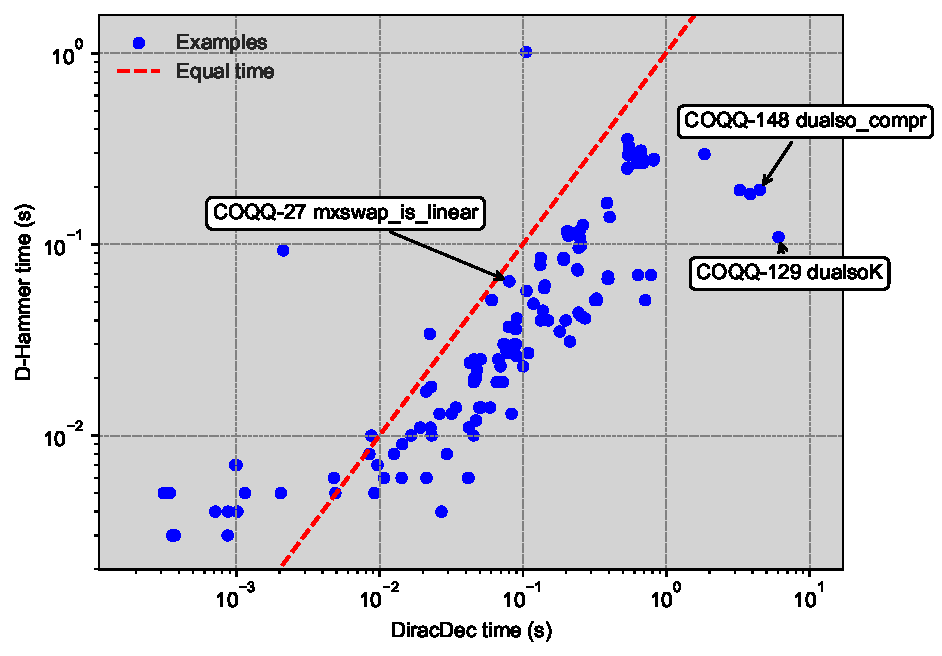
\includegraphics[width=0.65\textwidth]{fig/coqq.pdf}
    \caption{Time comparison between DiracDec and D-Hammer on the CoqQ benchmark.}
    \label{fig: CoqQ plot}
    \vspace{-0.4cm}
\end{figure}

\subsubsection{CoqQ}
As a more substantial example, we consider the examples from
CoqQ~\cite{Zhou2023}, an extensive formalization of quantum
information theory and quantum programming languages in the
Coq proof assistant.

CoqQ has been used as the main benchmark for evaluating DiracDec.
Specifically, \cite{diracdec} isolates 162 statements in CoqQ that
are in scope of the DiracDec language.

We have ported 158 out of 162 examples to D-Hammer. The remaining 4
examples uses projectors $\texttt{fst}$ and $\texttt{snd}$ on basis
pairs, where $\texttt{fst} (s, t) = s$ and $\texttt{snd} (s, t) =
t$. However, we found that this feature is rarely used and removed the
support in D-Hammer. Note that the omission of the projection rules
has a limited influence on the performance evaluation, because the
efficiency of the 158 examples is not affected by projection rules.

D-Hammer verifies the whole 158 examples in less than 10 seconds,
whereas DiracDec verifies 156/162 examples in more than 45 seconds.
\Cref{fig: CoqQ plot} shows a direct comparison of the efficiency of
the two tools. We observe that D-Hammer is slower than DiracDec on
small examples, due to marginal overhead, but becomes faster by an
average factor of 2 to 40 times as the running time of examples
increases. This non-linear growth suggests that efficiency gains
result from algorithmic improvements rather than the shift to a C++
implementation. Furthermore, examples with great improvements,
e.g. COQQ-129 and COQQ-148 shown in~\Cref{fig: CoqQ plot}, tend to use
deeply nested sums, for which our algorithm is more efficient.

 

% \subsubsection{Others}
% Other examples are taken from quantum circuits and one recent paper [TODO]. Because these examples involve decomposition on concrete $\ket{0}$ and $\ket{1}$ qubit basis, resulting a lot of addition elements, our algorithm dealing with AC symbols brings along significant improvement.
% One typical example is
% \begin{gather*}
%     (I \otimes P) \cdot U \cdot (I \otimes P) \cdot U^\dagger = \ket{0}\bra{0} \otimes I + \ket{1}\bra{1}\otimes (P \cdot P), \\
%     \textrm{where } P \triangleq e^{-i\theta/2} \ket{0}\bra{0} + e^{i\theta/2}\ket{1}\bra{1}, \qquad U \triangleq \ket{0}\bra{0} \otimes X + \ket{1}\bra{1} \otimes I.
% \end{gather*}
% It takes DiracDec about one minute, but D-Hammer solves it within one second.


\subsubsection{Labelled Dirac Notation}
We present a new set of examples for labelled Dirac notation (LDN), as illustrated in~\Cref{fig: labelled examples}. These examples include six representative cases drawn from various sources, such as well-established theorems, research paper results and quantum circuit equivalence.
D-Hammer successfully normalizes these examples and checks their equivalence using the algorithm outlined in~\Cref{sec: labelled}.
Among the examples, LDN-16 is a generalization of Example \ref{example1} and LDN-4 for Example \ref{ex: motivating}. LDN-12 shows the flexibility in combining labelled Dirac notations.
LDN-14 shows how to calculate controlled-not gate in different ways. 

A particularly noteworthy result is D-Hammer's solution to LDN-10, a highly complex and lengthy example. It is a theorem on quantum separation logic from~\cite{DBLP:conf/lics/ZhouBHYY21}, and proving it is challenging even for experts. Notably, it involves 7 registers, making it practically impossible to organize and referring to the subsystems without using labels.

\begin{figure}[h]
    \center
    % \scriptsize
    \setlength{\extrarowheight}{2pt}
    \begin{tabular}{l c c l}
        \hline
        example & source & time(s) & equation \\
        \hline
        LDN-4 & theorem & 0.03 & \( M_{r_1}\sum_{i}\ket{(i,i)}_{(r_1,r_2)} = M^T_{r_2}\sum_{i}\ket{(i,i)}_{(r_1, r_2)} \)\\
        LDN-10 & paper~\cite{DBLP:conf/lics/ZhouBHYY21} & 5.17 & \( \mathrm{tr}_{((a',(b,b')),c')}\Big[\mathrm{tr}_{r}\Big(U_{(r,(a,b))} \cdot\Big(|s\>_r\<s|\otimes 
        \Big[V_{((a',(b,b')),c')} \cdots \)\\
        LDN-11 & paper~\cite{PALSBERG2024206} & 0.12 & \( U_{(a,b)}\cdot W_{(b,c)}\cdot V_{(a,c)} = 
        \sum_i |i\>_a\<i|\otimes \big((P_i)_c\cdot W_{(b,c)}\cdot (Q_i)_c\big)\) \\
        LDN-12 & circuit & 0.07 & \( \ket{i}_{a;b}\bra{j} \cdot C_{(b,c)} \cdot D_{(c,d)} = {}_b\bra{j} \cdot C_{(b,c)} \cdot D_{(c,d)} \cdot \ket{i}_{a}\) \\
        LDN-14 & circuit & 7.37 & \scriptsize{\( \textsf{CNOT}_{rq}\ket{\textrm{GHZ}}_{pqr} = (\textsf{CNOT}\ket{00})_{rq}\ket{0}_p + (\textsf{CNOT}\ket{11})_{rq}\ket{1}_p \)} \\
        LDN-16 & theorem & 0.08 & \scriptsize{\( M_{prq}\ket{\textrm{GHZ}}_{prq} = N_{rq} \ket{\textrm{GHZ}}_{pqr}, M \triangleq \sum_{ij}\ket{ij}\bra{ij}\otimes U_{ij} \cdots \)} \\
        \hline
    \end{tabular}
    \caption{Part of examples for labelled Dirac notations. See~\Cref{sec: examples for labelled} for the full list.}
    \vspace{-0.2cm}
    \label{fig: labelled examples}
\end{figure}

\subsubsection*{Equivalence checking of circuits}
\gb{TODO}
